\chapter{Resultados e Análise}
\label{chap:resultados}

Este capítulo apresentará os resultados obtidos com a execução do Algoritmo de Grover em diferentes contextos computacionais: simulação ideal, simulação com ruído e execução real em hardware quântico. Os resultados são apresentados na forma de gráficos de distribuição de probabilidades dos estados finais, permitindo comparações qualitativas e quantitativas entre os cenários.

\section{Resultado Ideal (Teórico)}
\label{sec: resultIdeal}

Nesta seção, são apresentados os resultados obtidos a partir da simulação teórica ideal do circuito do Algoritmo de Grover, tal qual exemplificado na Figura~\ref{cod:simulacaoIdeol} da Seção~\ref{subSec: simulacaoIdeal}. Esta simulação permite visualizar a distribuição de probabilidades do estado final de maneira exata e sem influência de ruídos externos, funcionando como uma referência teórica para as demais simulações.

A Figura~\ref{fig:resultIdeal} mostra o histograma gerado após a aplicação do algoritmo, considerando um circuito com $4$ qubits e o estado marcado $\omega = \ket{1111}$. Observa-se que o algoritmo amplifica significativamente a probabilidade de ocorrência do estado marcado, como era esperado teoricamente.

\begin{figure}[ht!]
    \centering
    \captionsetup{justification=centering}
    \caption{ Distribuição Ideal de Probabilidades (Simulação via \texttt{Statevector}).}
    \label{fig:resultIdeal}
    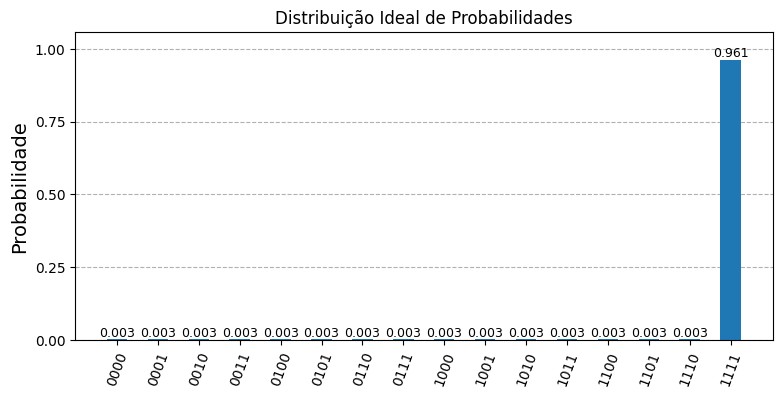
\includegraphics[width=.5\linewidth]{Imagens/resultIdeal.png}    
    
    {\small Fonte: do autor} 
\end{figure}

Com o valor ideal de iterações $k=3$ (resultado~\ref{eq:k = 3}), a probabilidade de medir o estado marcado $\ket{1111}$ foi de $96,1\%$, enquanto os demais estados apresentam probabilidades próximas de zero. Este comportamento é compatível com a expectativa teórica do algoritmo de Grover, conforme discutido nas seções anteriores e demonstrado também no Apêndice~\ref{ap:apendiceA}.

A distribuição obtida reflete, portanto, a eficiência máxima do algoritmo quando executado em condições ideais. Esta simulação serve como base de comparação para as análises subsequentes, em que serão incluídos fatores realistas como ruído, erro de leitura e imperfeições físicas presentes nos dispositivos quânticos atuais.

\section{Resultado com Ruído (\texttt{AerSimulator})}
\label{sec: resultRuido}

A simulação ideal apresentada na seção anterior assume um sistema quântico livre de ruídos. No entanto, implementações reais são afetadas por diversos tipos de erros, como decoerência, erro de porta, erro de leitura e ruído térmico. Para aproximar a execução do algoritmo à realidade dos dispositivos quânticos atuais, é necessário considerar esses fatores na simulação.

Esta seção tem por premissa a apresentação dos resultados da simulação feita usando dados de ruídos de dois \textit{backends} diferentes, já mencionados no Quadro~\ref{tab: backends}. Os modelos de ruídos são fornecidos pela classe \texttt{AerSimulator}, e podem ser utilizados como exemplificado na Figura~\ref{cod:simulacaoRuido} da Seção~\ref{subSec: simulacaoRuido}. Este modelo inclui características específicas e atuais do dispositivo real, como fidelidade de portas, taxas de erro de leitura e tempos de decoerência dos qubits, e por isso se faz uma ferramenta valiosa.

A Figura~\ref{fig:resultRuido} mostra o histograma da probabilidade final, em termos de porcentagem, de cada estado.

\begin{figure}[ht!]
    \centering
    \captionsetup{justification=centering}
    \caption{Distribuição de Probabilidades (Simulação via \texttt{AerSimulator}).}
    \label{fig:resultRuido}
    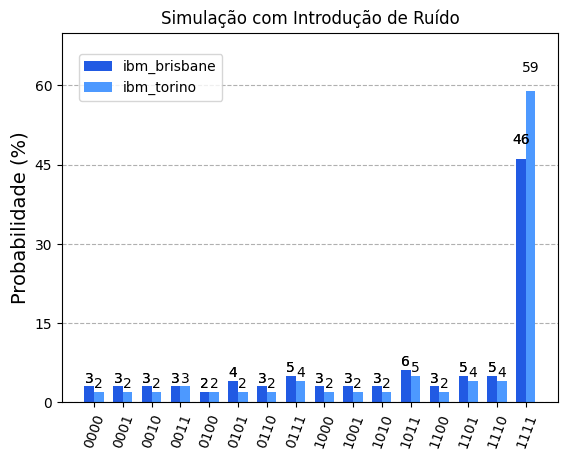
\includegraphics[width=.5\linewidth]{Imagens/resultRuido.png}    
    
    {\small Fonte: do autor} 
\end{figure}

Apesar da presença de ruído, observa-se que o estado marcado $\ket{1111}$ ainda possui a maior probabilidade entre os estados possíveis para ambos os modelos de ruído utilizados, com $46\%$ e $59\%$ para \textit{ibm\_brisbane} e \textit{ibm\_torino}, respectivamente. No entanto, pode-se notar facilmente que a presença do ruído, mesmo em ambiente simulado, já fornece um resultado bastante distorcido com relação à expectativa teórica (ou ideal), na qual a probabilidade para o estado marcado era superior a $96\%$. Ademais, os outros estados apresentam valores não desprezíveis, evidenciando a dispersão causada pelos erros quânticos.

\section{Resultado Real em \textit{Hardware} Quântico (\texttt{Sampler})}
\label{sec: resultReal}

Após a validação teórica e a simulação com ruído, o Algoritmo de Grover foi executado em dois computadores quânticos reais da \textit{IBM Quantum}: \textit{ibm\_brisbane} e \textit{ibm\_torino}, introduzidos na Seção~\ref{subSec: computadores}. A escolha de dois dispositivos teve como objetivo comparar o desempenho do mesmo circuito em arquiteturas físicas distintas, permitindo observar variações de fidelidade e impacto de parâmetros específicos de cada backend.

Para cada execução, foram configurados $20000$ \textit{shots}, e algumas condições específicas, conforme descritas abaixo:

\begin{enumerate}
    \item Sem nenhum método de supressão.
    \item \textit{Dynamical Decoupling} habilitado e \textit{Pauli Twirling} desabilitado.
    \item \textit{Dynamical Decoupling} desabilitado e \textit{Pauli Twirling} habilitado.
    \item Ambos habilitados.
\end{enumerate}

Esse mesmo padrão foi aplicado com dois níveis diferentes de otimização ($2$ e $3$). Todas essas diferentes preparações foram com o intuito de estudo e avaliação dos efeitos de cada método, inclusive quando aplicados simultaneamente.

A apresentação dos resultados é feita baseada nessas configurações, em que pode-se analisar em cada gráfico as diferenças causadas pelos métodos de supressão para um mesmo nível de otimização. Dito isso, a Figura~\ref{fig:resultBrisbane} mostra as quatro configurações de supressão aplicadas aos níveis de otimização $2$ e $3$ (Figuras~\ref{subfig:resultBrisbane_2} e~\ref{subfig:resultBrisbane_3}), enquanto a Figura~\ref{fig:resultTorino} replica as mesmas quatro configurações, também com os dois níveis de otimização aplicados a cada histograma (Figuras~\ref{subfig:resultTorino_2} e~\ref{subfig:resultTorino_3}). 

\begin{figure}[ht!]
    \centering
    \captionsetup{justification=centering}
    \caption{Resultados de \textit{ibm\_brisbane}.}
    \label{fig:resultBrisbane}

    \begin{subfigure}[b]{.46\textwidth}
        \centering
        \caption{Histograma de \textit{ibm\_brisbane} com $optim\_lvl = 2$}
        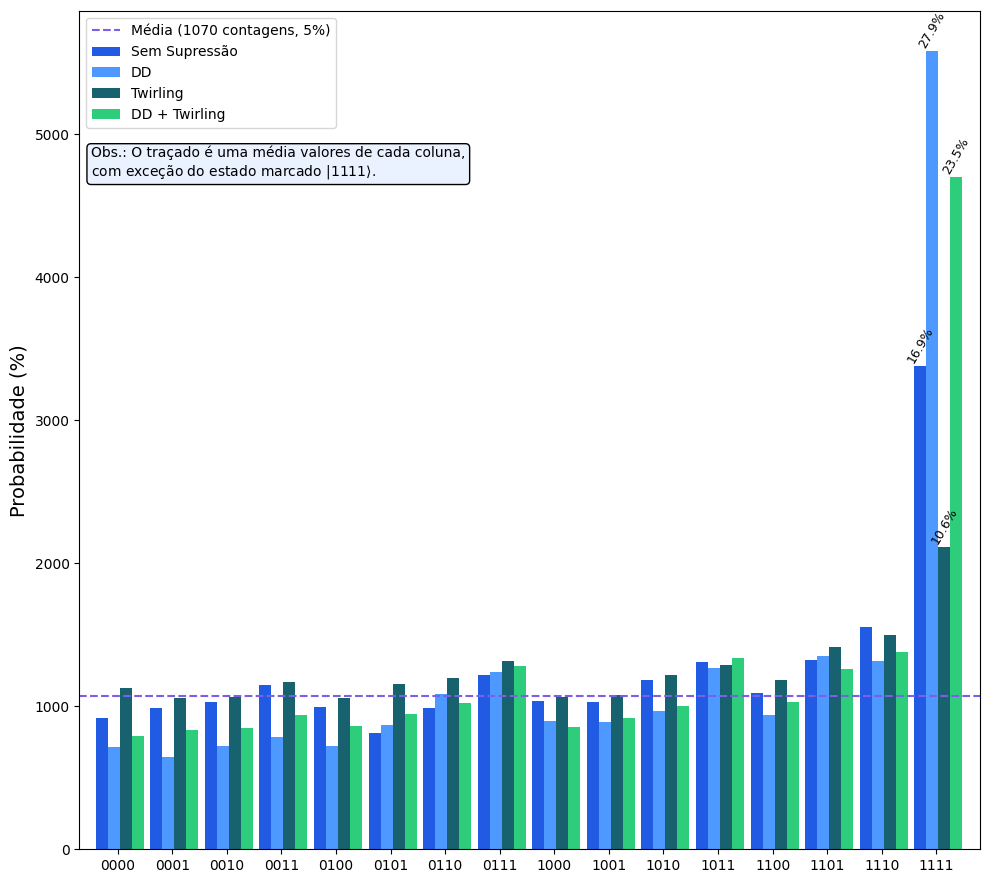
\includegraphics[width=\linewidth]{Imagens/resultBrisbane_2.png}
        \label{subfig:resultBrisbane_2}
    \end{subfigure}
    \hspace{1cm}
    \begin{subfigure}[b]{0.46\textwidth}
        \centering
        \caption{Histograma de \textit{ibm\_brisbane} com $optim\_lvl = 3$}
        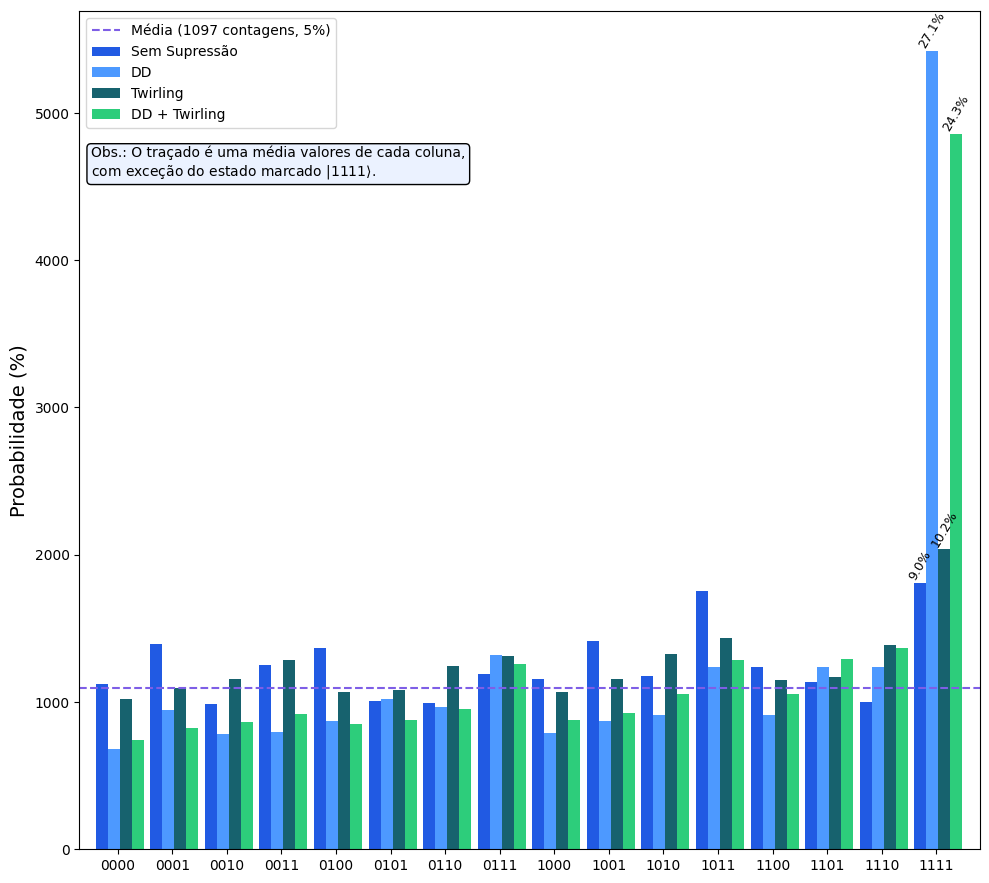
\includegraphics[width=\linewidth]{Imagens/resultBrisbane_3.png}
        \label{subfig:resultBrisbane_3}
    \end{subfigure}
    
    \vspace{0.3em}
    {\small Fonte: do autor} 
\end{figure}

\begin{figure}[ht!]
    \centering
    \captionsetup{justification=centering}
    \caption{Resultados de \textit{ibm\_torino}}
    \label{fig:resultTorino}

    \begin{subfigure}[b]{0.46\textwidth}
        \centering
        \caption{Histograma de \textit{ibm\_torino} com $optim\_lvl = 2$}
        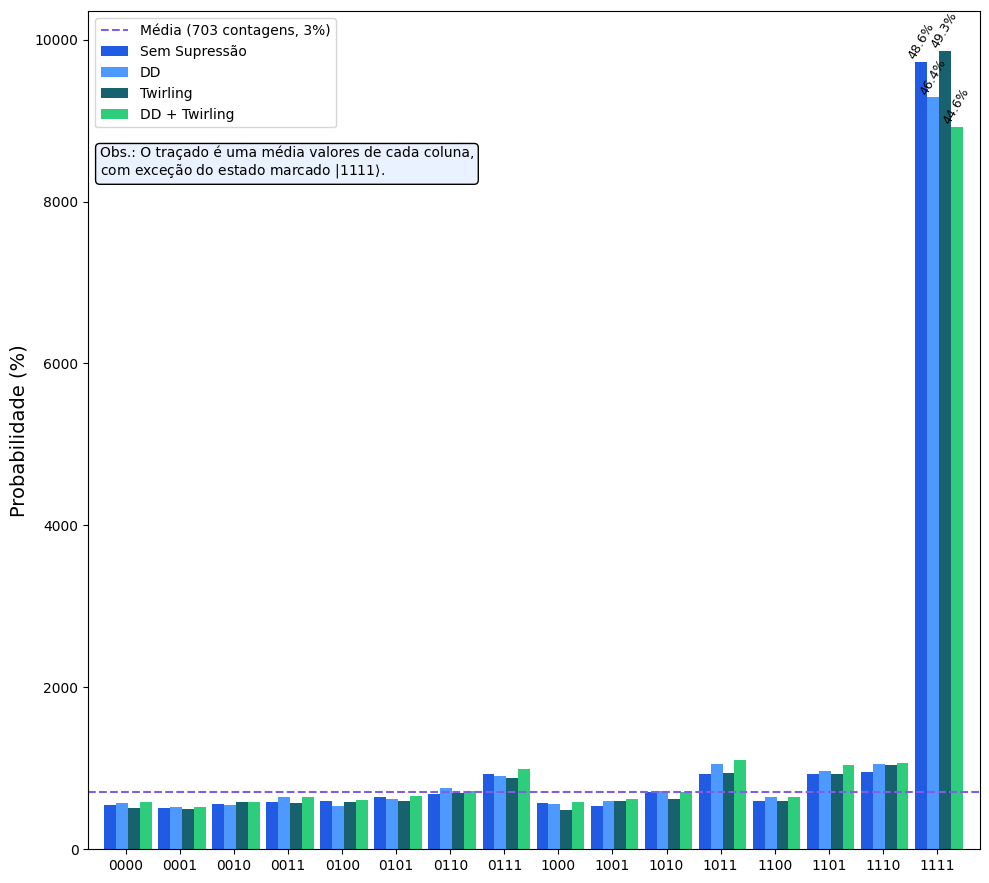
\includegraphics[width=\linewidth]{Imagens/resultTorino_2.png}
        \label{subfig:resultTorino_2}
    \end{subfigure}
    \hspace{1cm}
    \begin{subfigure}[b]{0.46\textwidth}
        \centering
        \caption{Histograma de \textit{ibm\_torino} com $optim\_lvl = 3$}
        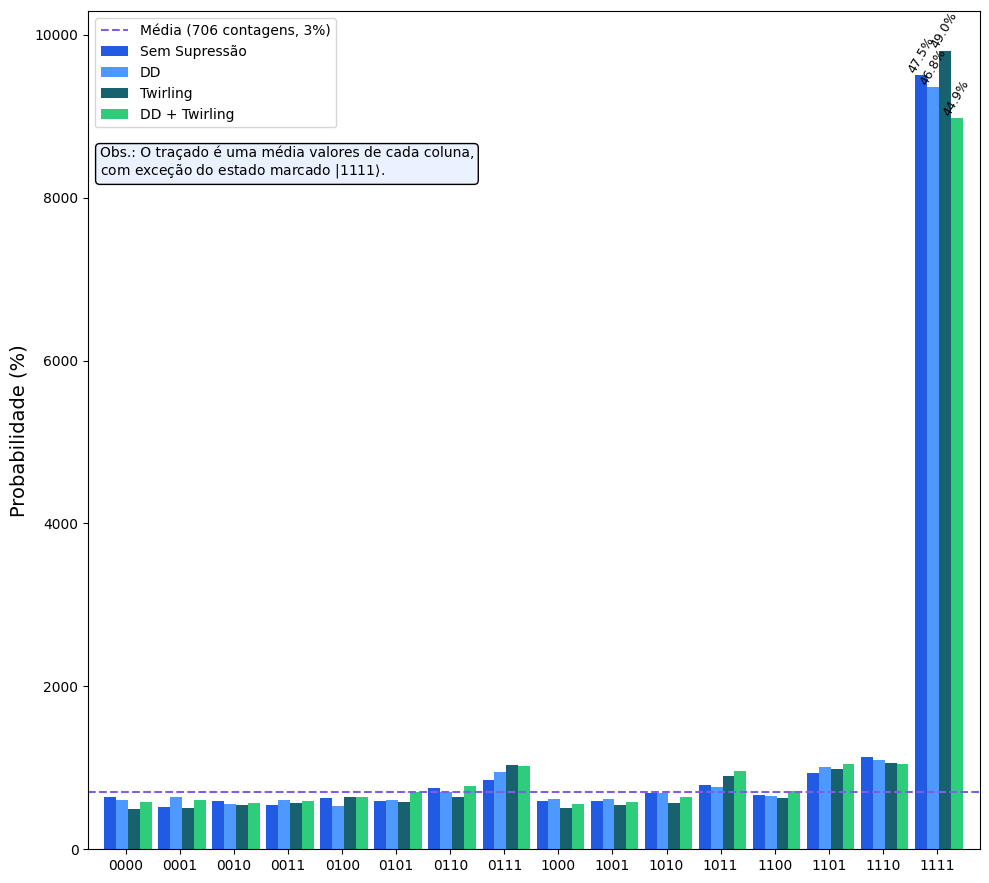
\includegraphics[width=\linewidth]{Imagens/resultTorino_3.png}
        \label{subfig:resultTorino_3}
    \end{subfigure}
    
    \vspace{0.3em}
    {\small Fonte: do autor} 
\end{figure}